\documentclass[journal,12pt,twocolumn]{IEEEtran}

\usepackage{setspace}
\usepackage{gensymb}
\singlespacing
\usepackage[cmex10]{amsmath}

\usepackage{amsthm}

\usepackage{mathrsfs}
\usepackage{txfonts}
\usepackage{stfloats}
\usepackage{bm}
\usepackage{cite}
\usepackage{cases}
\usepackage{subfig}

\usepackage{longtable}
\usepackage{multirow}

\usepackage{enumitem}
\usepackage{mathtools}
\usepackage{steinmetz}
\usepackage{tikz}
\usepackage{circuitikz}
\usepackage{verbatim}
\usepackage{tfrupee}
\usepackage[breaklinks=true]{hyperref}
\usepackage{graphicx}
\usepackage{tkz-euclide}

\usetikzlibrary{calc,math}
\usepackage{listings}
    \usepackage{color}                                            %%
    \usepackage{array}                                            %%
    \usepackage{longtable}                                        %%
    \usepackage{calc}                                             %%
    \usepackage{multirow}                                         %%
    \usepackage{hhline}                                           %%
    \usepackage{ifthen}                                           %%
    \usepackage{lscape}     
\usepackage{multicol}
\usepackage{chngcntr}

\DeclareMathOperator*{\Res}{Res}

\renewcommand\thesection{\arabic{section}}
\renewcommand\thesubsection{\thesection.\arabic{subsection}}
\renewcommand\thesubsubsection{\thesubsection.\arabic{subsubsection}}

\renewcommand\thesectiondis{\arabic{section}}
\renewcommand\thesubsectiondis{\thesectiondis.\arabic{subsection}}
\renewcommand\thesubsubsectiondis{\thesubsectiondis.\arabic{subsubsection}}


\hyphenation{op-tical net-works semi-conduc-tor}
\def\inputGnumericTable{}                                 %%

\lstset{
%language=C,
frame=single, 
breaklines=true,
columns=fullflexible
}
\begin{document}

\newcommand{\BEQA}{\begin{eqnarray}}
\newcommand{\EEQA}{\end{eqnarray}}
\newcommand{\define}{\stackrel{\triangle}{=}}
\bibliographystyle{IEEEtran}
\raggedbottom
\setlength{\parindent}{0pt}
\providecommand{\mbf}{\mathbf}
\providecommand{\pr}[1]{\ensuremath{\Pr\left(#1\right)}}
\providecommand{\qfunc}[1]{\ensuremath{Q\left(#1\right)}}
\providecommand{\sbrak}[1]{\ensuremath{{}\left[#1\right]}}
\providecommand{\lsbrak}[1]{\ensuremath{{}\left[#1\right.}}
\providecommand{\rsbrak}[1]{\ensuremath{{}\left.#1\right]}}
\providecommand{\brak}[1]{\ensuremath{\left(#1\right)}}
\providecommand{\lbrak}[1]{\ensuremath{\left(#1\right.}}
\providecommand{\rbrak}[1]{\ensuremath{\left.#1\right)}}
\providecommand{\cbrak}[1]{\ensuremath{\left\{#1\right\}}}
\providecommand{\lcbrak}[1]{\ensuremath{\left\{#1\right.}}
\providecommand{\rcbrak}[1]{\ensuremath{\left.#1\right\}}}
\theoremstyle{remark}
\newtheorem{rem}{Remark}
\newcommand{\sgn}{\mathop{\mathrm{sgn}}}
\providecommand{\abs}[1]{\vert#1\vert}
\providecommand{\res}[1]{\Res\displaylimits_{#1}} 
\providecommand{\norm}[1]{\lVert#1\rVert}
%\providecommand{\norm}[1]{\lVert#1\rVert}
\providecommand{\mtx}[1]{\mathbf{#1}}
\providecommand{\mean}[1]{E[ #1 ]}
\providecommand{\fourier}{\overset{\mathcal{F}}{ \rightleftharpoons}}
%\providecommand{\hilbert}{\overset{\mathcal{H}}{ \rightleftharpoons}}
\providecommand{\system}{\overset{\mathcal{H}}{ \longleftrightarrow}}
	%\newcommand{\solution}[2]{\textbf{Solution:}{#1}}
\newcommand{\solution}{\noindent \textbf{Solution: }}
\newcommand{\cosec}{\,\text{cosec}\,}
\providecommand{\dec}[2]{\ensuremath{\overset{#1}{\underset{#2}{\gtrless}}}}
\newcommand{\myvec}[1]{\ensuremath{\begin{pmatrix}#1\end{pmatrix}}}
\newcommand{\mydet}[1]{\ensuremath{\begin{vmatrix}#1\end{vmatrix}}}
\numberwithin{equation}{subsection}
\makeatletter
\@addtoreset{figure}{problem}
\makeatother
\let\StandardTheFigure\thefigure
\let\vec\mathbf
\renewcommand{\thefigure}{\theproblem}
\def\putbox#1#2#3{\makebox[0in][l]{\makebox[#1][l]{}\raisebox{\baselineskip}[0in][0in]{\raisebox{#2}[0in][0in]{#3}}}}
     \def\rightbox#1{\makebox[0in][r]{#1}}
     \def\centbox#1{\makebox[0in]{#1}}
     \def\topbox#1{\raisebox{-\baselineskip}[0in][0in]{#1}}
     \def\midbox#1{\raisebox{-0.5\baselineskip}[0in][0in]{#1}}
\vspace{3cm}
\title{ EE3900 : Assignment-3}
\author{Nelakuditi Rahul Naga - AI20BTECH11029}
\maketitle
\newpage
\bigskip
\renewcommand{\thefigure}{\theenumi}
\renewcommand{\thetable}{\theenumi}
Download all python codes from 
\begin{lstlisting}
https://github.com/Rahul27n/EE3900/blob/main/Assignment_3/Assignment_3.py
\end{lstlisting}
%
and latex-tikz codes from 
%
\begin{lstlisting}
https://github.com/Rahul27n/EE3900/blob/main/Assignment_3/Assignment_3.tex
\end{lstlisting}
\vspace{0.5cm}
\section{QUESTION: RAMSEY 4.2 TANGENT AND NORMAL Q.16}
Find the equations of the circles that touch the lines:
\begin{align}
\myvec{0 & 1}\vec{x} &= 0 \label{eq:1}
\\\myvec{0 & 1}\vec{x} &= 4 \label{eq:2}
\\\myvec{2 & 1}\vec{x} &= 2 \label{eq:3}
\end{align}
\section{SOLUTION}
The general equation of a circle can be expressed as:
\begin{align}
\vec{x^T}\vec{x} + 2\vec{u^T}\vec{x} + f = 0 \label{eq:4}
\end{align}
If $r$ is radius and $\vec{c}$ is the centre of the circle we have:
\begin{align}
f &=\vec{u}^T\vec{u}-r^2  \label{eq:5} \\  
\vec{c} &=-\vec{u}
\end{align}

Let the circles of the form \eqref{eq:4} touch the lines \eqref{eq:1} and \eqref{eq:2} (which are \textbf{parallel}) at general points $\vec{M}$ and $\vec{N}$ given by:
\begin{align}
\vec{M} &= \myvec{m \\ 0}\\
\vec{N} &= \myvec{n \\ 4}
\end{align} 
respectively.

We note that the common normal of \eqref{eq:1} and \eqref{eq:2} passing through the centre of the circle is of the form :
\begin{align}
\myvec{1 & 0}\vec{x}=k 
\end{align}
where $k$ is a constant.

Now $\vec{M}$ and $\vec{N}$ lie on the aforementioned common normal. Hence we have:
\begin{align}
\myvec{1 & 0}\myvec{m \\ 0} &= k\\
\implies m= k\\
\myvec{1 & 0}\myvec{n \\ 4} &= k\\
\implies n= k
\end{align}

The centre $\vec{c}$ of the circle must be the mid-point of $\vec{M}$ and $\vec{N}$ as $\vec{M}$ and $\vec{N}$ are the touch points of parallel tangents to a circle. Therefore we have:
\begin{align}
\vec{c} &= \dfrac{\myvec{m \\ 0} + \myvec{n \\ 4}}{2}\\
\vec{c} &= \dfrac{\myvec{k \\ 0} + \myvec{k \\ 4}}{2}\\
\vec{c} &= \myvec{k \\ 2}
\end{align}

Also the radius $r$ of the circles is given by:
\begin{align}
r &= \dfrac{\norm{\vec{M}-\vec{N}}}{2}
&= \dfrac{\sqrt{(k-k)^{2}+(0-4)^{2}}}{2}\\
r &= 2
\end{align}

From \eqref{eq:5} we have:
\begin{align}
f &=\myvec{-k&-2}\myvec{-k\\-2}-r^2\\
f &= k^2 + 2^2 -2^2\\
f &= k^2\label{eq:6}
\end{align}
The equation of the remaining line is
\begin{align}
\myvec{2 & 1}\vec{x}& = 2 \label{eq:7}
\end{align}

The general equation of a second degree can be expressed as :
\begin{align}
\vec{x}^T\vec{V}\vec{x}+2\vec{u}^T\vec{x}+f=0\label{eq:8}
\end{align}

The points of contact $\vec{q}$, of a line with a normal vector $\vec{n}$ to the conics in \eqref{eq:8} are given by:
\begin{align}
\vec{q} = \vec{V}^{-1}\brak{\kappa \vec{n}-\vec{u}} \label{eq:9} \\
\kappa = \pm \sqrt{\frac{\vec{u}^T\vec{V}^{-1}\vec{u}-f}{\vec{n}^T\vec{V}^{-1}\vec{n}}}\label{eq:10}
\end{align}
We know that, for a circle, 
\begin{align}
\vec{V} = \vec{I}\label{eq:11}  
\end{align}
and from the properties of an Identity matrix, 
\begin{align}
\vec{I}^{-1} &= \vec{I} \\
\vec{I}\vec{X} &= \vec{X}   
\end{align}
From \eqref{eq:5}, \eqref{eq:7} and \eqref{eq:11} we have:
\begin{align}
\kappa &= \pm \sqrt{\frac{r^2}{\myvec{2 & 1 }\myvec{2 \\ 1 }}} \\
&= \pm \sqrt{\frac{4}{5}} \\
& =  \pm \frac{2}{\sqrt{5}}
\end{align}
Therefore from \eqref{eq:9} we have:
\begin{align}
\vec{q} &= \pm \myvec{\dfrac{4}{\sqrt{5}} \\ \dfrac{2}{\sqrt{5}} } - \myvec{-k \\ -2} \\
&=\myvec{\dfrac{\pm 4}{\sqrt{5}} +k \\\dfrac{\pm 2}{\sqrt{5}} +2}
\end{align}

Now $\vec{q}$ lies on the line \eqref{eq:7} therefore,
\begin{align}
\myvec{2 & 1}\myvec{\dfrac{\pm 4}{\sqrt{5}} +k \\\dfrac{\pm 2}{\sqrt{5}} +2} &= 2 \\
2\Bigg(\dfrac{\pm 4}{\sqrt{5}} +k\Bigg) + \Bigg(\dfrac{\pm 2}{\sqrt{5}} +2\Bigg) &= 2\\\
2k = \pm \dfrac{10}{\sqrt{5}}\\
\implies k = \pm \sqrt{5} \\
\implies f = k^2 = 5
\end{align}
Hence the tangent circles are given by the equations:
\begin{align}
\vec{x^T}\vec{x} + \myvec{2\sqrt{5} & -4}\vec{x} + 5 &= 0 \\
\vec{x^T}\vec{x} + \myvec{-2\sqrt{5} & -4}\vec{x} + 5 &= 0
\end{align}
The illustration of the circles and the lines is shown below :
\begin{figure}[!ht]
       \centering
    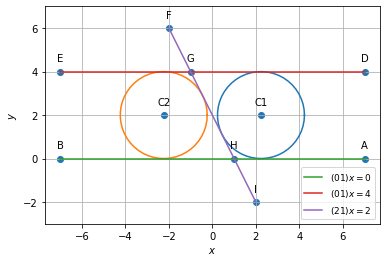
\includegraphics[width=\columnwidth] {Assignment_3_Fig_1.png}
    \caption{Circles touching given lines with centres C1,C2}
    \label{Tangent circles to 3 given lines}
\end{figure}

\end{document}